\chapter{Technology Review}

\section{GitHub}
GitHub is a Version Control Software that stores the entire code history of projects in what they call 'Repositories' (Figure 3.1), with READMEs and Wikis in Markdown for documentation. Repositories can be used for individual usage, and they can add collaborators to commit (contribute) to the repository. For team-based usage, an organization can be created that would contain individual repositories that all team members can commit to the repository. It is an amazing tool. With GitHub, if something went wrong with a project, e.g. a bug or a sudden loss of files, they can all be recovered from the repository making it easier and faster to fix problems. It gives the opportunity to show off work their users have done to future employers without having to send ZIP files or screenshots. GitHub was widely used in this project, from the repository to the projects board and the issues. It was a wise choice for the project and should be enforced a lot more to use in other modules for projects/assignments.

\begin{figure}[H]
    \caption{Repota App Repository}
    \label{image:gitRepo}
    \centering
    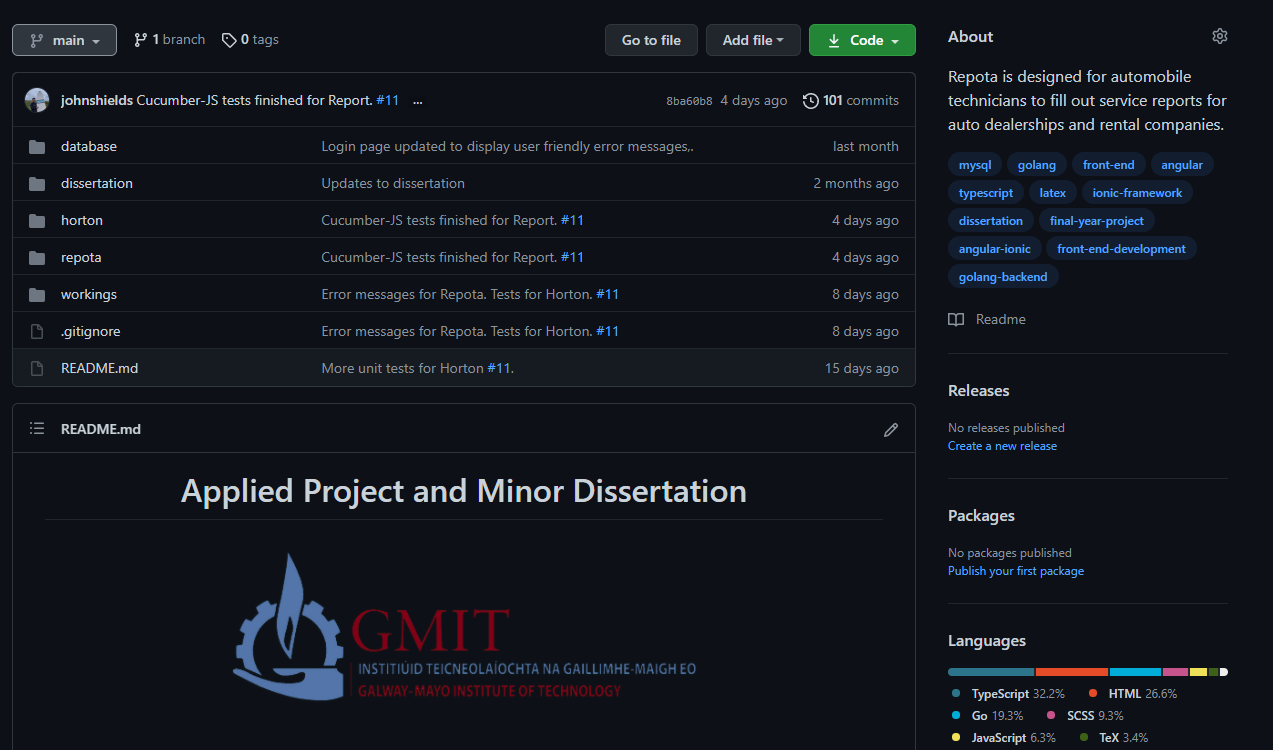
\includegraphics[width=0.7\textwidth]{images/misc/git-repo.png}
\end{figure}

\section{OpenAPI}
OpenAPI specification are machine-readable API blueprints for RESTful web services. Client and Server stubs can be generated along with documentation just from these blueprints. OpenAPI enables to perfect with an efficiency of design and testing. Swagger Tools allow for the implementation of specifications for these blueprints. These blueprints can be written in YAML, which is in a human-readable format. 

Swagger Tools was highly used for prototyping the project's, server, and client stubs along with their Schema Models. With Swagger, server stubs can be easily designed with the necessary HTTP requests and responses. To follow the server's stubs, the client stubs get generated with the inter-grated design to allow it to talk back and forth to the server. Swagger made the process of designing the project's OpenAPI specification a structured and straightforward task. It proved to be extremely useful and easy to use for a first-time user.

\begin{figure}[H]
    \caption{OpenAPI Spec - Swagger Editor}
    \label{image:swaggerEditor}
    \centering
    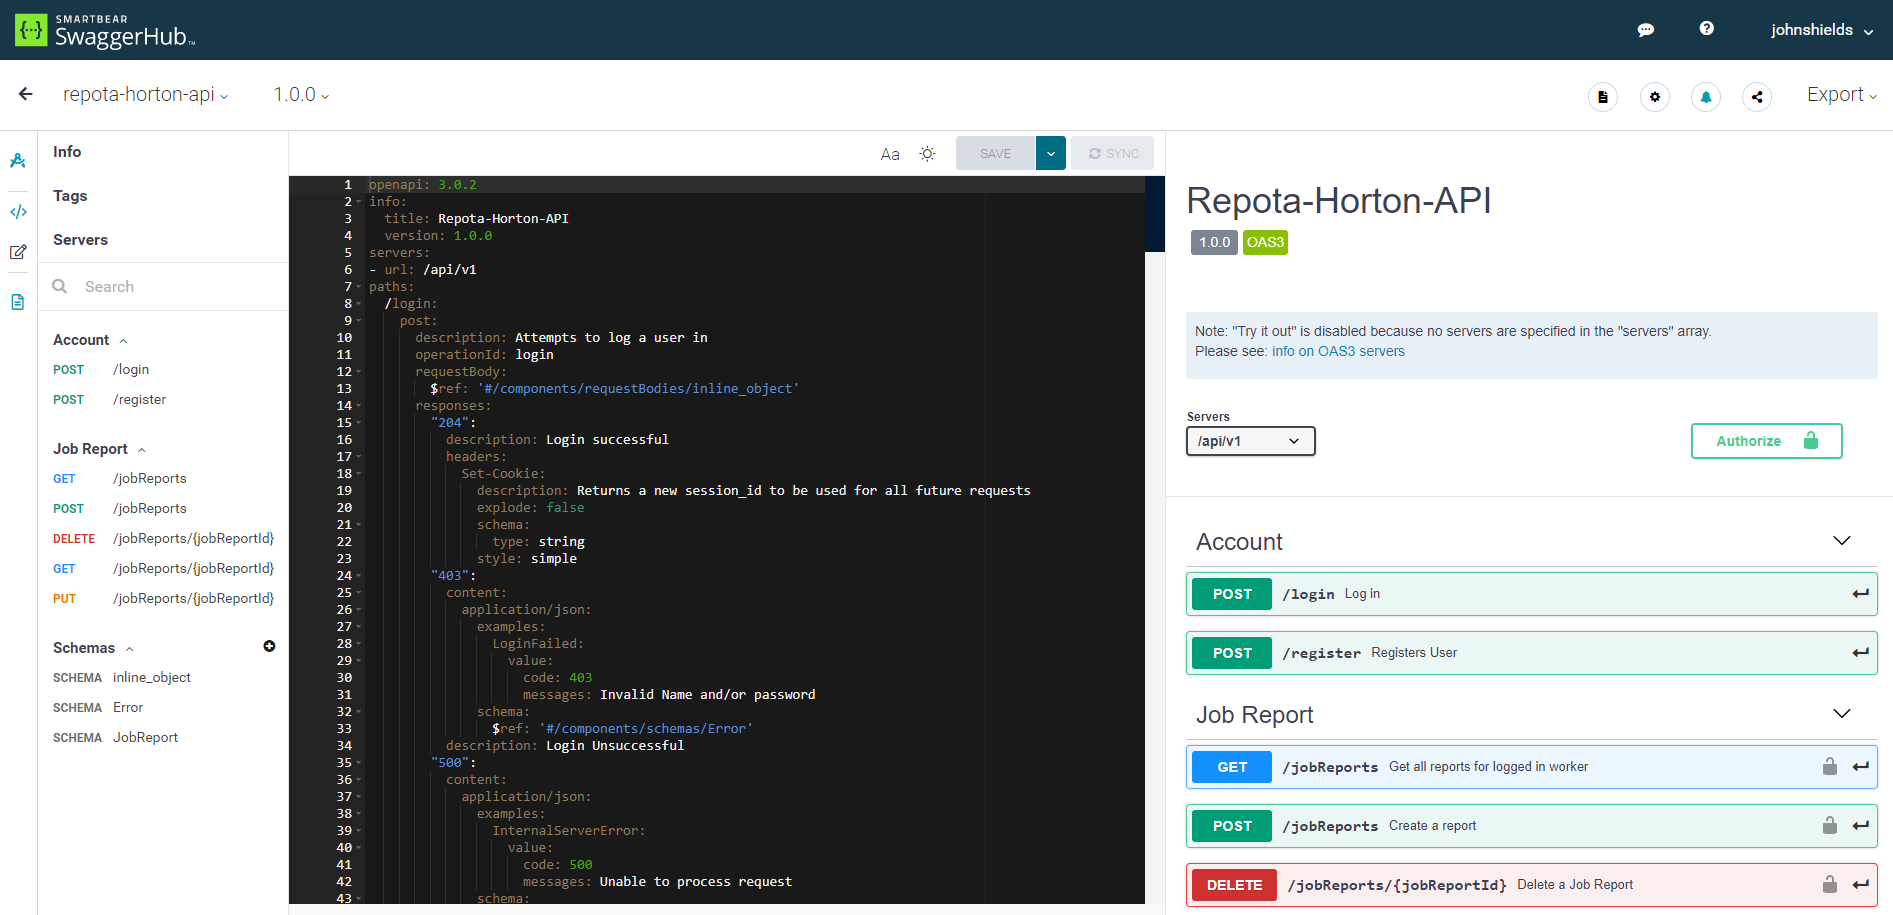
\includegraphics[width=1.0\textwidth]{images/misc/openapi.png}
\end{figure}

\begin{figure}[H]
    \caption{Schema Models - Swagger Editor}
    \label{image:swaggerSchemas}
    \centering
    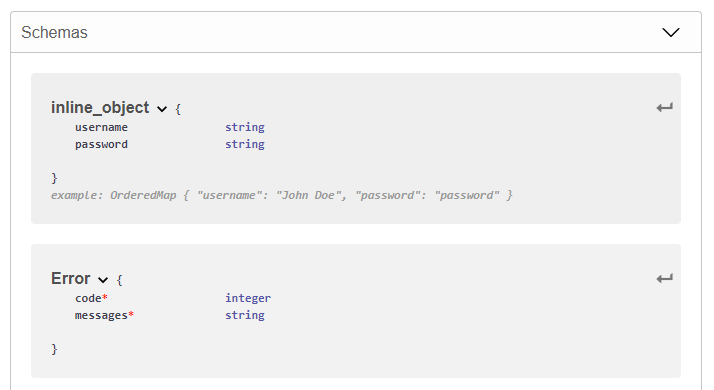
\includegraphics[width=0.7\textwidth]{images/misc/swagger-schemas.png}
\end{figure}

\section{Golang}
Golang (Go), designed by Google, is an loosely based Object-Oriented Programming (OOP) Language. Go is a relatively new language (first version released on November 10, 2009), open-source and becoming widely used. Go is primarily based on the C programming language and has compile speeds that can be as fast as Java and C++ (See Figure 3.4). \cite{ref6} When it comes to OOP, Go is especially great for refactoring and abstraction. Go does not uses classes like Java, the closest thing to a class in Go is a Struct. \cite{ref7} Go files can pick up functions from others easily as long they are in the same package. A function can be taken from one file and be put into another and still be able to be picked up in the original file with no changes or additions. If a function is in another package, it can easily be used outside with an import of that package and a variable declaring that function. 

\begin{figure}[H]
    \caption{Go VS Java \& C++ \cite{ref6}}
    \label{image:goJavaCpp}
    \centering
    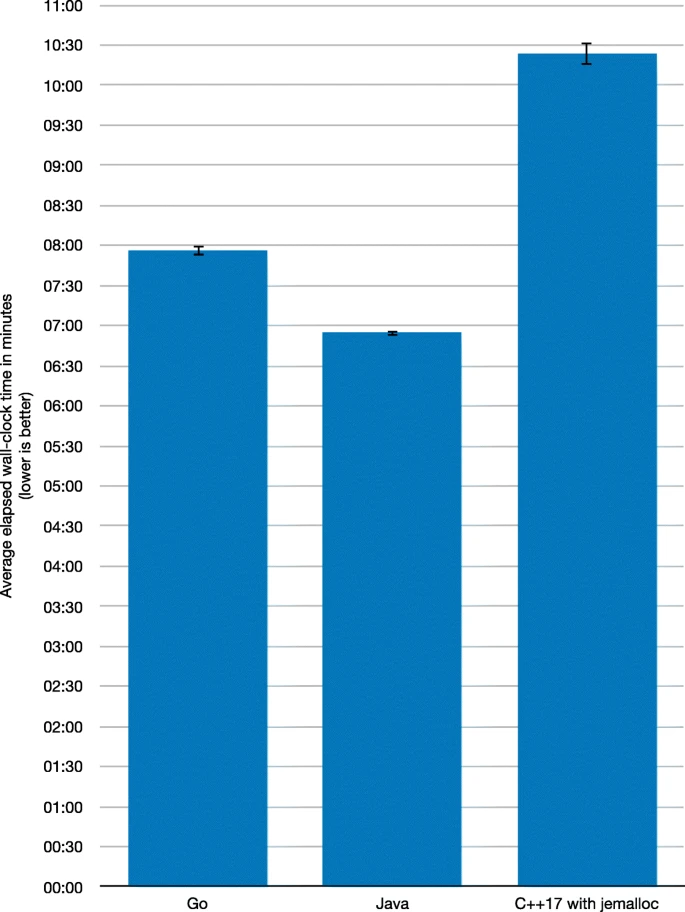
\includegraphics[width=0.5\textwidth]{images/misc/go-java-cpp.png}
\end{figure}

The main idea of Go is to reduce the development of large servers with big machines, many cores, and developers and bring it down to the use of simple tools that can do all those jobs. Identifying problems in Go is a more straightforward process as the tools are simple, allowing concentrating on the problem rather than how to solve it. With the Go SDK installation (Software Development Kit), Go's documentation can be accessed through the CLI (Command Line Interface). For example, simply typing the command 'go doc fmt' into the CLI lists all the documentation on formatting print statements (Figure 3.4). Go doc can also be used to list all the functions inside a project's package (Figure 3.5). With the command 'godoc -http=:6060', a localhost of Go's complete documentation can be accessed, which would provide great use if there is a weak/no internet connection.

\begin{figure}[H]
    \caption{CLI Go Docs on fmt}
    \label{image:goDocFmt}
    \centering
    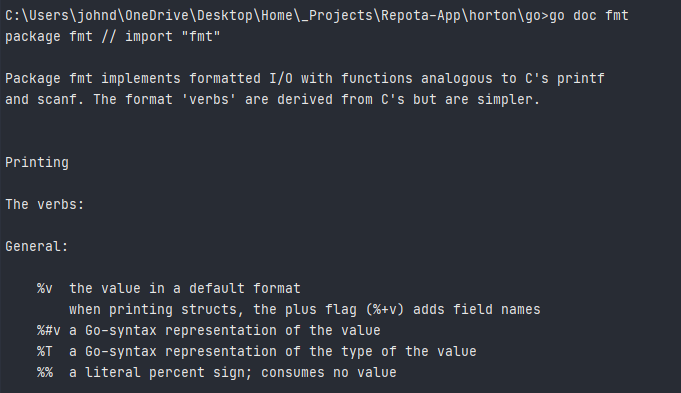
\includegraphics[width=1.0\textwidth]{images/misc/go-doc-fmt.png}
\end{figure}

\begin{figure}[H]
    \caption{Go Functions inside the Back-end's openapi Package}
    \label{image:goFuncs}
    \centering
    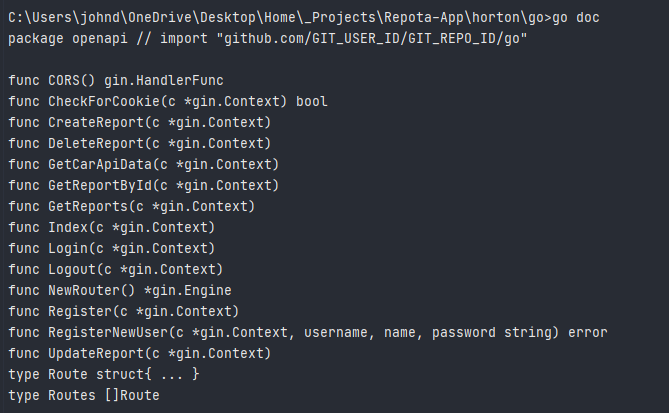
\includegraphics[width=1.0\textwidth]{images/misc/godoc-funcs.png}
\end{figure}

\subsection{Go Web Frameworks}
\subsubsection{Gorilla Mux}
Gorilla Mux is a package that implements a request router and dispatcher for assigning incoming requests to the appropriate handler. Mux stands for "HTTP request multiplexer". mux.ServeMux is similar to http.ServeMux. Incoming requests are compared to a list of registered routes, and the path that meets the URL or other requirements. \cite{ref8} 

\subsubsection{Gin Gonic}
Gin Gonic has a Martini-like API but with an efficiency that is up to 40 times faster. Martini is another Go web framework, which is no longer maintained. Gin is fast, "Radix tree-based routing, small memory footprint. No reflection. Predictable API performance." A chain of middle-wares can handle incoming HTTP requests. Gin's error management makes it simple to gather all of the errors during a HTTP search. Gin allows the creation of custom HTTP responses errors (Figure 3.7). If a panic occurs in an HTTP request, Gin can recover it, making it "Crash-free". \cite{ref9} 

There is a limitation with Gin. Endpoints sharing a common path may result in issues. For example 'api/movies/:movieId' and 'api/movies/:releaseDate' will result in a issue with gin. Having colliding paths in APIs is common, and they can usually switch over and back, but with Gin, they can not. However, depending on the paths required for an API, if the paths are for basic CRUD operations (CREATE, READ, UPDATE AND DELETE), this should not be much of an issue. It becomes an issue when an API needs multiple operations other than CRUD which, Gin does not meet the requirements. 

\begin{figure}[H]
    \caption{Gin Error Handling}
    \label{image:ginError}
    \centering
    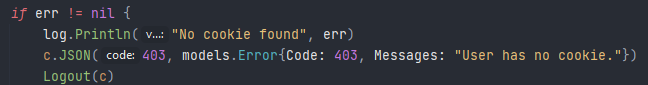
\includegraphics[width=1.0\textwidth]{images/misc/cookie-error.png}
\end{figure}

\subsection{How Go fitted the Back-end}
Back-ends can be developed in many languages, including Java, Python, Ruby, Node.js, and Rust. Go stood out from the others for the Back-end for how it handles compile times, syntax, documentation, its use of OOP and seemed like a great language to learn. 

Learning Go for the first time for the Back-end was a welcome challenge. It took some time to become comfortable and with the use of 'go doc' made that process smooth. The central part of this challenge was finding a suitable Web Framework that had all the requirements needed. Gorilla Mux was used for the prototype but failed to meet the requirements to deal this CORS.
Gin Gonic proved to be the best framework to use, but it required Docker to generate the OpenAPI stubs for Gin rather than Swagger's standard options. After finalizing the Back-end, it can be said that Go is a very nice language. 
 
\section{Angular \& Ionic}
There are many JavaScript and TypeScript frameworks out there, including Angular, React, Vue.js, Meteor, Ember.js, ETC. These technologies are primarily JavaScript frameworks. A new JavaScript framework almost appears every year. Some of these frameworks can become obsolete as there is always a new one coming right around the corner.

Angular is a TypeScript-based web app framework and with the combination of Ionic can make web apps into mobile apps. Angular is relatively slow to run apps, but they can be updated once they are up and running without having to rerun them. Angular apps are created with components, and Ionic turns them into pages. The figure below shows the structure of a page.

\begin{figure}[H]
    \caption{Angular \& Ionic Home Page Structure}
    \label{image:ngHomePage}
    \centering
    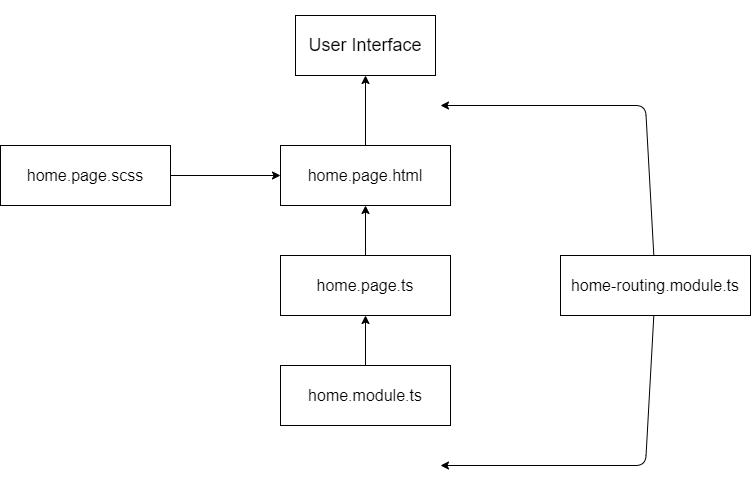
\includegraphics[width=0.8\textwidth]{images/misc/ng-homepage.png}
\end{figure}

\textbf{UI Structure and Styling}
\begin{itemize}
    \item home.page.html \& home.page.scss
\end{itemize} 

\textbf{Controller of UI: Buttons, Input boxes ETC.}
\begin{itemize}
    \item home.page.ts 
\end{itemize} 

\textbf{Imports and Dependencies}
\begin{itemize}
    \item home.module.ts
\end{itemize} 

\textbf{Path Routing to connect the page to the App's main routing}
\begin{itemize}
    \item home-routing.module.ts
\end{itemize} 

\subsection{Routing}
When an Angular and Ionic app is first initialized, template pages are setup. Every page has a routing module that connects to the main app routing module (app-routing.module.ts). This module allows for complete access to navigation through routes. For example, the home page would be on the www.app.com/home route (Figure 3.9). These routing endpoints are similar to what a RESTful API would use.

\begin{figure}[H]
    \caption{Route of Repota's Home Page}
    \label{image:homeRoute}
    \centering
    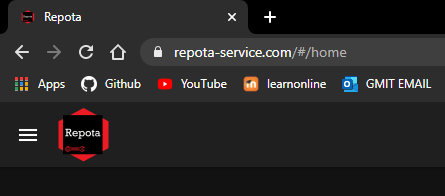
\includegraphics[width=0.8\textwidth]{images/misc/home-route.png}
\end{figure}

\subsection{How Angular \& Ionic fitted the Front-end}
Before this project Angular and Ionic were used in the past to create apps for other modules and personal interest. Meaning that these frameworks were chosen for their comfort-ability and have been successful for other projects. The main reason why an uncomfortable app framework was not chosen as it was thought that learning and becoming component with a new language for the back-end was more important and would be more useful beyond college. Ionic did proved to be very useful as it immensely helped make the front-end responsive for mobile phones using the mobile phone simulator Ionic Lab. 

\section{MySQL}
MySQL is a database management system for relational databases (RBMS) that use the ACID model. It is the most common open-source database in the world because it is efficient, simple to set up, and use. \cite{ref10} MySQL is quite robust, both in it's setup for database tables and its functionality.
 
 \subsection{Relational}
 Rather than storing all of the data in one big storeroom, a relational database stores it in different tables. Physical files are used to organize the database structures, which are designed for pace. The logical model provides a versatile programming environment with artifacts such as databases, tables, views, rows, and columns. \cite{ref11}
 
 \subsection{ACID}
The ACID model is a collection of database design principles that place a premium on aspects of reliability that are crucial for business data and mission-critical applications. ACID stands for Atomicity, Consistency, Isolation, and Durability. Atomicity is used in InnoDB transactions with statements such as 'COMMIT' and 'ROLLBACK'. Transactions are a way of updating multiple tables at one time (See Figure 3.10). Transactions are usually used when two tables are connected by the use of foreign keys. Consistency protects data from crashes by having transactions broken down into parts. When several transactions are making adjustments and running queries simultaneously, Isolation fine-tunes the balance between efficiency and reliability, accuracy, and reproducibility of results. Finally, Durability which, stores only the successful transactions in the database. \cite{ref12}
 
 \begin{figure}[H]
    \caption{MySQL InnoDB Transaction for inserting data into two tables.}
    \label{image:transaction}
    \centering
    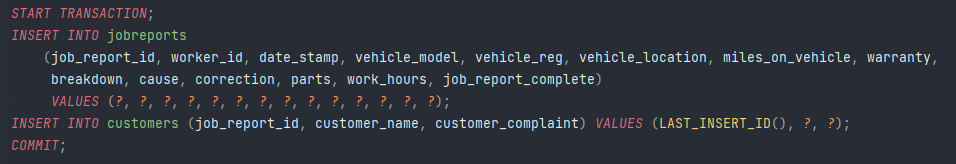
\includegraphics[width=1.0\textwidth]{images/misc/mysql-transation.png}
\end{figure}

\subsection{How MySQL fitted the Database}
MySQL was chosen for many reasons. MySQL definitely seemed like the best fit. As discussed in the introduction, Repota is designed for vehicle technicians (workers). In a database, workers need their own dedicated table. For any app, website, system for a company of any sort, there needs to be storage for their workers. If the data were all in one place, it would be a mess, and worker information would get lost right in the middle of it. Having separate, connected tables for data was a necessity for the project. Workers are stored in one table. That table then connects to the service reports table which, is then connected to the customers' table. Keeping dedicated tables for workers and customers was seen as a must as their information if very important for the service reports.

Given that the reports consist of report and customer information, transactions are perfect to create new reports without hassle. MySQL 'JOIN QUERIES' allow selecting data from multiple tables to present the data as if all the data was originally in one table. Since the complete reports consist of data from two other tables, JOIN QUERIES were the way to go. From these observations, it was quite obvious, MySQL was perfect for the database. 

\section{Amazon Web Services}
Amazon Web Services (AWS) is a cloud platform with many services. Some of these services are EC2, Route 53, Machine Learning, Elastic Beanstalk, S3 Bucket, and CloudFront. Deploying to AWS can be as simple as uploading source code files. AWS has its own CLI which, generally works better for deployment. Uploading files can overload the service. Should a significant update needed to be deployed, previous files would first need to be deleted before uploading any new files. With AWS's CLI, command modifiers such as '--delete' can be used during deployment. This modifier deletes any files and deploys the updated ones with ease.

\subsection{Virtual Machines}
A Virtual Machine (VM) is a virtualization or emulation of a computer. VMs allow having a Linux Operating System (OS) accessible from the CLI of a Windows computer with no installation needed. From the Windows side, the connection is generally made in a PowerShell or GIT Bash CLI. AWS's EC2 (Elastic Compute Cloud) service handles VMs. EC2 provides the service to have many VMs with different operating systems.

\subsubsection{Windows VS Linux}
Since Windows OS is a commercial product, only the developers who developed it have the authority to alter it. The Linux operating system is open-source, allowing users to configure their environments to their taste. Linux is considered to be faster than the most recent Windows versions. Linux is extremely stable because it is simple to find and repair bugs, and in contrast, Windows is vulnerable to viruses and malware because of its vast user base. \cite{ref13}

\subsection{S3 Bucket}
S3 (Simple Storage Service) provides object storage. Objects are the fundamental entities stored in S3. With S3 Bucket, web apps can be stored and hosted. To deploy/upload to a Bucket source code files can be upload or with the AWS CLI. By default, these Buckets are HTTP, meaning they are not secure for data transfers. Buckets can become secure (HTTPS) using AWS's Route 53, Certificate Manager, and CloudFront. Route 53 allows to setup hosted zones for a custom web domain. Route 53 takes a domain and routes it to an AWS service such as a S3 Bucket or an Elastic Beanstalk. With CloudFront, that custom domain can become secure. Certificate Manager can issue SSL (Secure Sockets Layer) certificates to domains. That SSL certificate can then be set up with CloudFront. From here, Route 53 can then be used to point the Bucket to the secure CloudFront domain.

\subsection{Elastic Beanstalk}
Elastic Beanstalk (EB) is a service for deploying and scaling web apps and services. These web apps and services are usually developed in Java, .NET, PHP, Node.js Python, Go, and Docker. Docker can be used through EB. The addition of Docker and the EB CLI makes deploying to EB a satisfying process. Similar to S3 Buckets EBs are HTTP by default. HTTP can be overcome with a somewhat similar process to making a Bucket secure. In the EB configuration settings, a load balancer can be set up to be on a HTTPS port with a SSL certificate. Then Route 53 can be used to point a custom domain to that EB. EB uses Environments to host web apps. These environments have logs to access console outputs, warnings, or information from the web app.

\subsubsection{Docker}
Docker is a set of platform-as-a-service products that use OS-level virtualization to deliver applications in 'containers', as Docker refers to them. A container is a file format for packaging software that encapsulates all of an app's code and dependencies in a standard format that allows it to run quickly and efficiently across multiple computing environments.

\subsection{How AWS fitted the project's hosting}
AWS seemed like the best fit for hosting as it manages its services very well. The UI itself is well structured and easy to navigate for a cloud platform with several services. The project's database needed to be on a secure server. AWS's EC2 service was opted for the database, hosted on a secure Ubuntu VM. Initially, the project's back-end was also hosted on this VM for prototyping reasons. When the back-end's structure was finalized, it deployed to EB through Docker. Once the front-end had its core functionality it was hosted through AWS's S3 Bucket. The back-end and front-end are both HTTPS thanks to AWS's Route 53, CloudFront, and Certificate Manager.

